%++++++++++++++++++++++++++++++++++++++++
\documentclass[article, 12pt]{article}
\usepackage{float}
\usepackage{setspace}
\usepackage{tabu} % extra features for tabular environment
\usepackage{amsmath}  % improve math presentation
\usepackage{graphicx} % takes care of graphic including machinery
\usepackage[margin=1in]{geometry} % decreases margins
\usepackage{cite} % takes care of citations
\usepackage[final]{hyperref} % adds hyper links inside the generated pdf file
\usepackage{tikz}
\usepackage{caption} 
\usepackage{fancyhdr}
\usepackage{amssymb} % symbols like /therefore
\usepackage{amsthm} % proofs
\usepackage{enumerate} % lettered lists
\usepackage{mathtools} % macros
\usepackage[ all]{xy} % for diagrams
\usetikzlibrary{scopes}
% \usepackage{xcolor} \pagecolor[rgb]{0.12549019607,0.1294117647,0.13725490196} \color[rgb]{0.82352941176,0.76862745098,0.62745098039} % dark theme
\theoremstyle{definition}
\newtheorem{example}{Example}[subsubsection]
\newtheorem*{remark}{Remark}
\newtheorem{theorem}{Theorem}[subsubsection]
\newtheorem{definition}{Definition}[subsubsection]
\newtheorem{corollary}{Corollary}[subsubsection]
\hypersetup{
	colorlinks=false,      % false: boxed links; true: colored links
	linkcolor=blue,        % color of internal links
	citecolor=blue,        % color of links to bibliography
	filecolor=magenta,     % color of file links
	urlcolor=blue         
}
\usepackage{physics}
\usepackage{siunitx}
\usepackage{tikz,pgfplots}
\usepackage[outline]{contour} % glow around text
\usetikzlibrary{calc}
\usetikzlibrary{angles,quotes} % for pic
\usetikzlibrary{arrows.meta}
\tikzset{>=latex} % for LaTeX arrow head
\contourlength{1.2pt}

\colorlet{xcol}{blue!70!black}
\colorlet{vcol}{green!60!black}
\colorlet{myred}{red!70!black}
\colorlet{myblue}{blue!70!black}
\colorlet{mygreen}{green!70!black}
\colorlet{mydarkred}{myred!70!black}
\colorlet{mydarkblue}{myblue!60!black}
\colorlet{mydarkgreen}{mygreen!60!black}
\colorlet{acol}{red!50!blue!80!black!80}
\tikzstyle{CM}=[red!40!black,fill=red!80!black!80]
\tikzstyle{xline}=[xcol,thick,smooth]
\tikzstyle{mass}=[line width=0.6,red!30!black,fill=red!40!black!10,rounded corners=1,
                  top color=red!40!black!20,bottom color=red!40!black!10,shading angle=20]
\tikzstyle{faded mass}=[dashed,line width=0.1,red!30!black!40,fill=red!40!black!10,rounded corners=1,
                        top color=red!40!black!10,bottom color=red!40!black!10,shading angle=20]
\tikzstyle{rope}=[brown!70!black,very thick,line cap=round]
\def\rope#1{ \draw[black,line width=1.4] #1; \draw[rope,line width=1.1] #1; }
\tikzstyle{force}=[->,myred,very thick,line cap=round]
\tikzstyle{velocity}=[->,vcol,very thick,line cap=round]
\tikzstyle{Fproj}=[force,myred!40]
\tikzstyle{myarr}=[-{Latex[length=3,width=2]},thin]
\def\tick#1#2{\draw[thick] (#1)++(#2:0.12) --++ (#2-180:0.24)}
\DeclareMathOperator{\sn}{sn}
\DeclareMathOperator{\cn}{cn}
\DeclareMathOperator{\dn}{dn}
\def\N{80} % number of samples in plots


\usepackage{titling}
\renewcommand\maketitlehooka{\null\mbox{}\vfill}
\renewcommand\maketitlehookd{\vfill\null}
\usepackage{siunitx} % units
\usepackage{verbatim} 
\newcommand{\courseNumber}{MATH 263}
\newcommand{\courseName}{Discrete Mathematics 2}
\newcommand{\professor}{Dr. Petrescu}
\newcommand{\psetName}{Homework 1B}
\newcommand{\dueDate}{Due: February 10, 2023}
\newcommand{\name}{Denny Cao}
\pagestyle{fancy}
\fancyhf{}% clears all header and footer fields
\fancyfoot[C]{--~\thepage~--}
\renewcommand*{\headrulewidth}{0.4pt}
\renewcommand*{\footrulewidth}{0pt}
\lhead{\name}
\chead{\courseNumber: \courseName}
\rhead{\professor}
\newcounter{questionNumber}
\newcommand{\question}[1]{\stepcounter{questionNumber}\noindent\textbf{Problem \arabic{questionNumber}:} #1}
\newcommand{\answer}[1]{\noindent\textbf{Answer:} #1}

\fancypagestyle{plain}{%
  \fancyhf{}% clears all header and footer fields
  \fancyfoot[C]{--~\thepage~--}%
  \renewcommand*{\headrulewidth}{0pt}%
  \renewcommand*{\footrulewidth}{0pt}%
}

% Shortcuts
\DeclarePairedDelimiter\ceil{\lceil}{\rceil} % ceil function
\DeclarePairedDelimiter\floor{\lfloor}{\rfloor} % floor function

\DeclarePairedDelimiter\paren{(}{)} % parenthesis

\newcommand{\df}{\displaystyle\frac} % displaystyle fraction
\newcommand{\qeq}{\overset{?}{=}} % questionable equality

\newcommand{\Mod}[1]{\;\mathrm{mod}\; #1} % modulo operator

\newcommand{\comp}{\circ} % composition

% Sets
\DeclarePairedDelimiter\set{\{}{\}}
\newcommand{\unite}{\cup}
\newcommand{\inter}{\cap}

\newcommand{\reals}{\mathbb{R}} % real numbers: textbook is Z^+ and 0
\newcommand{\ints}{\mathbb{Z}}
\newcommand{\nats}{\mathbb{N}}
\newcommand{\rats}{\mathbb{Q}}

\newcommand{\degree}{^\circ}

% Counting
\newcommand\perm[2][^n]{\prescript{#1\mkern-2.5mu}{}P_{#2}}
\newcommand\comb[2][^n]{\prescript{#1\mkern-0.5mu}{}C_{#2}}

% Relations
\newcommand{\rel}{\mathcal{R}} % relation

\setlength\parindent{0pt}

% Directed Graphs
\usetikzlibrary{arrows}
\tikzset{vertex/.style = {shape=circle,draw,minimum size=1.5em}}
\tikzset{edge/.style = {->,> = latex'}}

% Sign Charts
\newdimen\tcolw \tcolw=2.5em % the column width
\edef\ecatcode{\catcode`&=\the\catcode`&\relax}\catcode`&=4
\def\sgchart#1#2{\vbox{\offinterlineskip\halign{\hfil##\quad&##\hfil\crcr\sgchartA#2,:,%
   \omit\sgchartR&\kern.2pt\sgchartS{.5\tcolw}\relax\sgchartE#1,\relax,%
   \sgchartS{.5\tcolw}\relax\cr
   \noalign{\kern2pt}&\def~{}\kern.5\tcolw\sgchartD#1,\relax,\cr}}}
\def\sgchartA#1:#2,{\cr\ifx,#1,\else $#1$&\sgchartB#2{}\expandafter\sgchartA\fi}
\def\sgchartB#1{\hbox to\tcolw{\hss$#1$\hss}\sgchartC}
\def\sgchartC#1{\ifx,#1,\else
   \strut\vrule\kern-.4pt\hbox to\tcolw{\hss$#1$\hss}\expandafter\sgchartC\fi}
\def\sgchartD#1#2,{\ifx\relax#1\else\hbox to\tcolw{\hss$#1#2$\hss}\expandafter\sgchartD\fi}
\def\sgchartE#1#2,{\ifx\relax#1\else
    \ifx~#1\sgchartS\tcolw\circ \else\sgchartS\tcolw\bullet\fi \expandafter\sgchartE\fi}
\def\sgchartR{\leaders\vrule height2.8pt depth-2.4pt\hfil}
\def\sgchartS#1#2{\hbox to#1{\kern-.2pt\sgchartR \ifx\relax#2\else
   \kern-.7pt$#2$\kern-.7pt\sgchartR\fi\kern-.2pt}}
\ecatcode
%++++++++++++++++++++++++++++++++++++++++
% title stuff

\makeatletter
\renewcommand{\maketitle}{\bgroup\setlength{\parindent}{0pt}
    \begin{flushleft}
        \textbf{\@title} \\ \vskip0.2cm
        \begingroup
            \fontsize{14pt}{12pt}\selectfont
            \courseNumber: \courseName 
            \vskip0.3cm **
            \professor
        \endgroup \vskip0.3cm
        \@date \hfill\rlap{}\bf{\name} \\ \vskip0.1cm
        \hrulefill
    \end{flushleft}\egroup 
}
\makeatother

\title{\Huge\bf{\psetName}}
\author{\name}
\date{\dueDate}

\author{\name}
\date{\dueDate}

\begin{document}
    \maketitle
    \thispagestyle{empty}

    % Question 1
    \question{Determine whether the relation given by the digraph below is an equivalence relation. Justify your answer.

    \begin{figure}[H]
        \centering
        \xygraph{ !{<0cm,0cm>;<3cm,0cm>:<0cm,3cm>::} !{(0,0);a(0)**{}?(1.0)}*+[red]{\bullet_{a}}="a" !{(0,0);a(72)**{}?(1.0)}*+[blue]{\bullet_{b}}="b" !{(0,0);a(108)**{}?(0.5)}*+[red]{\bullet_{c}}="c" !{(0,0);a(216)**{}?(1.0)}*+[green]{\bullet_{d}}="d" !{(0,0);a(288)**{}?(1.0)}*+[red]{\bullet_{e}}="e" !{(0,0);a(0)**{}?(1.8)}*+{\bullet_{f}}="f" !{(0,0);a(72)**{}?(1.8)}*+[blue]{\bullet_{g}}="g" !{(-1,0);a(144)**{}?(1.8)}*+[blue]{\bullet_{h}}="h" !{(0,0);a(252)**{}?(.8)}*+[green]{\bullet_{i}}="i" !{(0,0);a(288)**{}?(1.8)}*+[green]{\bullet_{j}}="j" "a":"c""c":@/^1cm/"a""c":"e""e":@/^1cm/"c" "a":@/_1cm/"e""e":"a""c":@/^1cm/"f" "g":"h" "b":"h" "i":"h" "j":"i" "j":"f" "a":"f"  "f":@/^.2cm/"a" "b":"g" "j":"d" "j":"e" "d":"h" "i":@/_.6cm/"d" "j":@/^4.6cm/"h" "d":"i" "e":@/_.5cm/"f" "f":"e""a":@(ru,rd)"a""b":@(ru,rd)"b" "c":@(lu,ld)"c""d":@(ld,lu)"d""e":@(ru,rd)"e" "f":@(ru,rd)"f""g":@(ru,rd)"g" "h":@(lu,ld)"h" "i":@(lu,ld)"i""j":@(ru,rd)"j" "h":@/_.2cm/"d""h":@/_.4cm/"i""h":@/_6cm/"j" "f":@/_.2cm/"j""g":@/_.4cm/"b""h":@/_.6cm/"b""h":@/_.8cm/"g""d":@/_.8cm/"j""i":@/_.8cm/"j" "e":@/_.2cm/"j"}
    \end{figure}}

    \begin{proof}
        The relation is not an equivalence relation. $aRf$ and $fRj$, but $a\not R j$. Thus, the relation is not a transitive relation, and therefore is not an equivalence relation, as equivalence relations must be reflexive, symmetric, and transitive.
    \end{proof}
    % Question 2
    \question{Determine whether the relation given by the digraph below is a partial order.  If it is, draw its Hasse diagram.

    \begin{figure}[H]
        \centering
        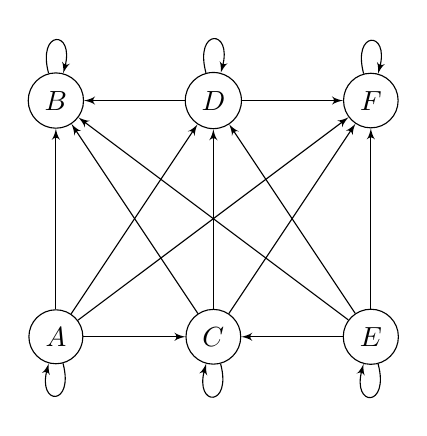
\begin{tikzpicture}

            \node[vertex] (a) at (0,0) {$A$};
            \node[vertex] (b) at (0,3) {$B$};
            \node[vertex] (c) at (2,0) {$C$};
            \node[vertex] (d) at (2,3) {$D$};
            \node[vertex] (e) at (4,0) {$E$};
            \node[vertex] (f) at (4,3) {$F$};
            
            \draw[edge] (a) to[loop below] (a);
            \draw[edge] (a) to (b);
            \draw[edge] (a) to (c);
            \draw[edge] (a) to (d);
            \draw[edge] (a) to (f);
        
            \draw[edge] (b) to[loop above] (b);
        
            \draw[edge] (c) to[loop below] (c);
            \draw[edge] (c) to (b);
            \draw[edge] (c) to (d);
            \draw[edge] (c) to (f);
        
            \draw[edge] (d) to[loop above] (d);
            \draw[edge] (d) to (b);
            \draw[edge] (d) to (f);
            
            \draw[edge] (e) to[loop below] (e);
            \draw[edge] (e) to (b);
            \draw[edge] (e) to (c);
            \draw[edge] (e) to (d);
            \draw[edge] (e) to (f);
        
            \draw[edge] (f) to[loop above] (f);
            \end{tikzpicture}
    \end{figure}}

    \begin{proof}
        The relation is a partial order, as it as reflexive, antisymmetric, and transitive. 

        The relation is reflexive, as $\forall x \in \{A, B, C, D, E, F\}(xRx)$. This can be seen by observing that all of the vertices are connected to themselves.
        \\[12pt]
        The relation is antisymmetric, as $\forall x \forall y \in \{A, B, C, D, E, F\}(xRy \to y \not \rel x)$. This can be seen by observing that there are no bidirectional edges.

        The relation is transitive, as $\forall x \forall y \forall z \in \{A, B, C, D, E, F\}(xRy \land yRz \to xRz)$. 
    \end{proof}
    \begin{figure}[H]
        \centering
        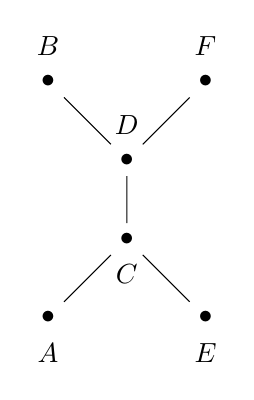
\begin{tikzpicture}
            \node[label=below:$A$] (a) at (0,0) {$\bullet$};
            \node[label=above:$B$] (b) at (0,3) {$\bullet$};
            \node[label=below:$C$] (c) at (1,1) {$\bullet$};
            \node[label=above:$D$] (d) at (1,2) {$\bullet$};
            \node[label=below:$E$] (e) at (2,0) {$\bullet$};
            \node[label=above:$F$] (f) at (2,3) {$\bullet$};
            
            \draw (a) -- (c) -- (d) -- (b);
            \draw (e) -- (c);
            \draw (d) -- (f);
        
        \end{tikzpicture}
    \end{figure}

    % Question 3
    \question{What is the transitive closure of the relation $R=\{(1, 2), (1, 4), (2, 3), (3, 1), (4, 2)\}$?}
    The original relation can be represented by the following matrix:
    \begin{equation*}
        R^0 = \begin{bmatrix}
            0 & 1 & 0 & 1 \\
            0 & 0 & 1 & 0 \\
            1 & 0 & 0 & 0 \\
            0 & 1 & 0 & 0 \\
        \end{bmatrix}
    \end{equation*}
        We apply Warshall's method to find the transitive closure of the relation:
        \begin{align*}
            R^1 &= \begin{bmatrix}
                0 & 1 & 0 & 1 \\
                0 & 0 & 1 & 0 \\
                1 & 1 & 0 & 1 \\
                0 & 1 & 0 & 0 \\
            \end{bmatrix} \quad
            R^2 = \begin{bmatrix}
                0 & 1 & 1 & 1 \\
                0 & 0 & 1 & 0 \\
                1 & 1 & 1 & 1 \\
                0 & 1 & 1 & 0 \\
            \end{bmatrix}
            \\
            R^3 &= \begin{bmatrix}
                0 & 1 & 1 & 1 \\
                0 & 0 & 1 & 0 \\
                1 & 1 & 1 & 1 \\
                0 & 1 & 1 & 0 \\	
            \end{bmatrix} \quad
            R^4 = \begin{bmatrix}
                0 & 1 & 1 & 1 \\
                0 & 1 & 1 & 0 \\
                1 & 1 & 1 & 1 \\
                0 & 1 & 1 & 0 \\
            \end{bmatrix}
        \end{align*}
    \\[12pt]
    % Question 4
    \question{Show that the relation $R = \{(x, y) | x - y \in \mathbb{Z} 	\}$ is an equivalence relation on the set of rational numbers. What are the equivalence classes of 0 and $\frac12$?}
    
\end{document} 
